\documentclass[border=10pt]{standalone}
\usepackage{tikz}
\usetikzlibrary{shapes.geometric, arrows.meta, positioning, fit, backgrounds}

\begin{document}
	
	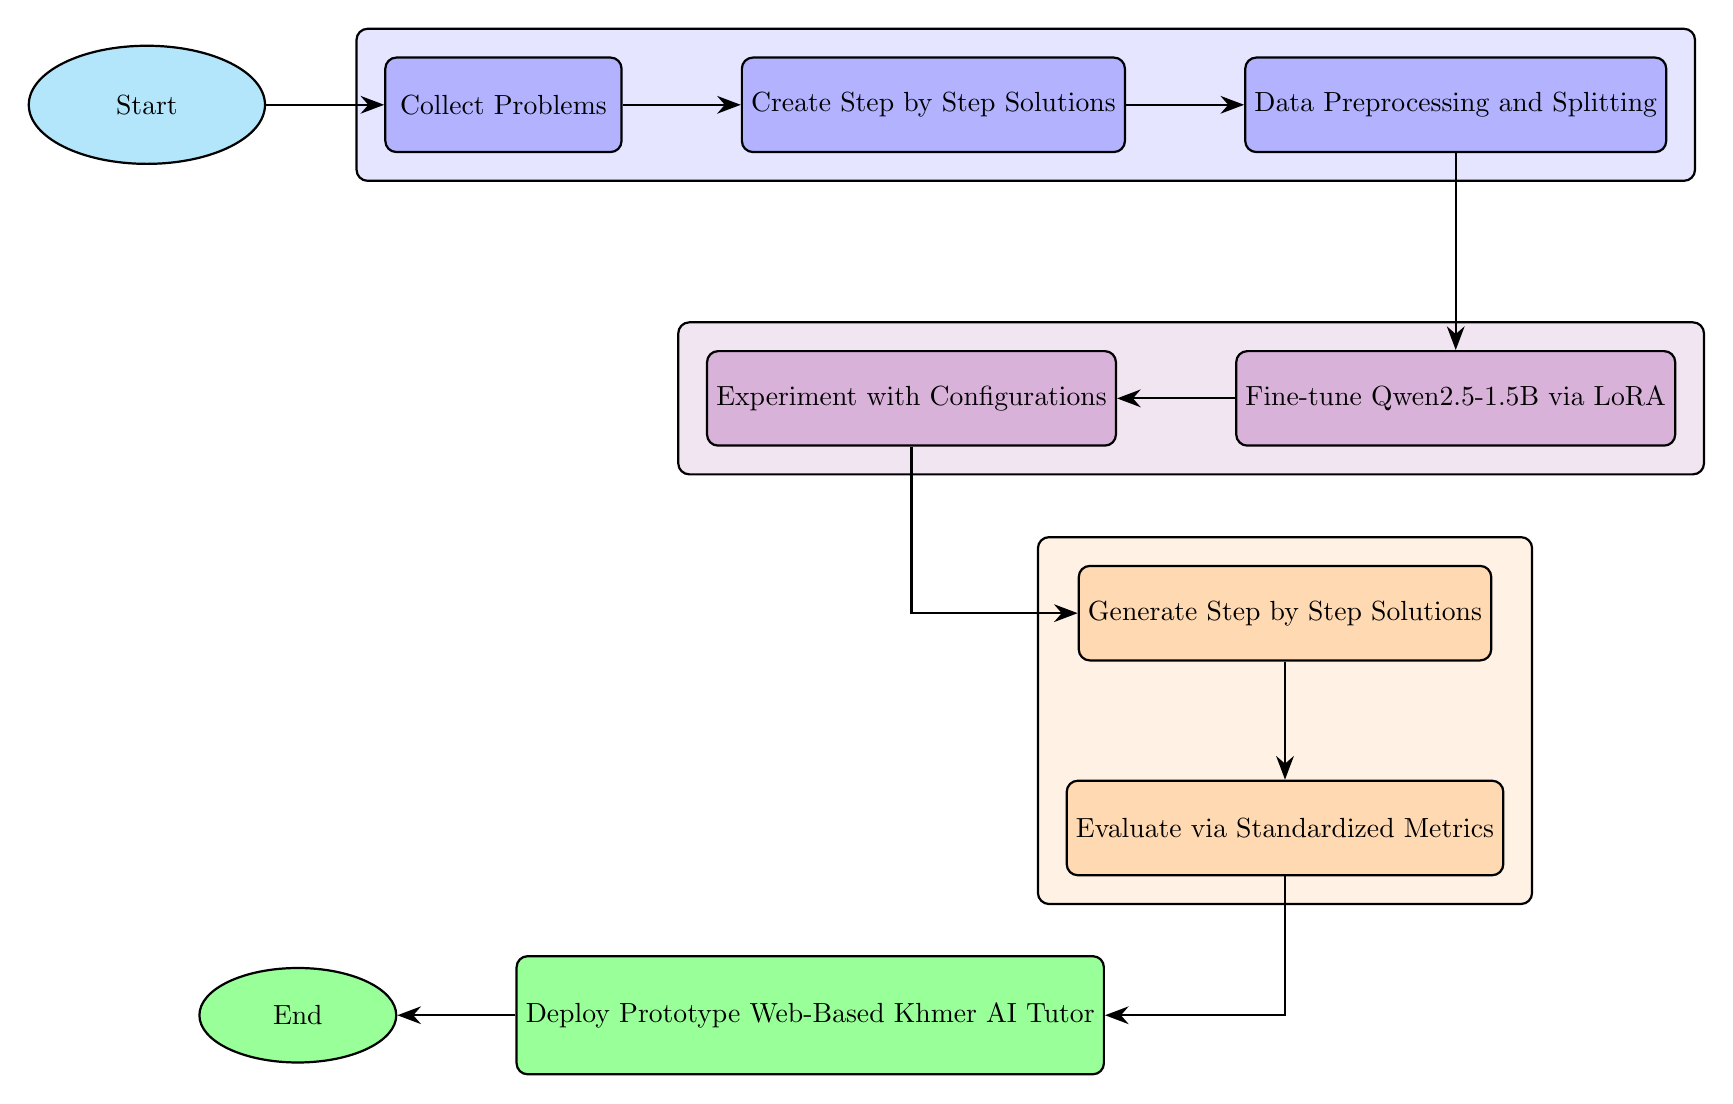
\begin{tikzpicture}[
		node distance=1.5cm,
		auto,
		% Define styles
		startstop/.style={ellipse, minimum width=3cm, minimum height=1.5cm, text centered, draw=black, fill=cyan!30, thick},
		process/.style={rectangle, minimum width=3cm, minimum height=1.2cm, text centered, draw=black, fill=blue!30, thick, rounded corners},
		process2/.style={rectangle, minimum width=3cm, minimum height=1.2cm, text centered, draw=black, fill=violet!30, thick, rounded corners},
		process3/.style={rectangle, minimum width=3cm, minimum height=1.2cm, text centered, draw=black, fill=orange!30, thick, rounded corners},
		deploy/.style={rectangle, minimum width=3.5cm, minimum height=1.5cm, text centered, draw=black, fill=green!40, thick, rounded corners},
		endstyle/.style={ellipse, minimum width=2.5cm, minimum height=1.2cm, text centered, draw=black, fill=green!40, thick},
		arrow/.style={thick,-{Stealth[length=3mm]}},
		dashedarrow/.style={thick,-{Stealth[length=3mm]}, dashed},
		container/.style={rectangle, draw, thick, rounded corners, inner sep=10pt}
		]
		
		% Start node
		\node (start) [startstop] {Start};
		
		% Dataset Development section
		\node (collect) [process, right=of start] {Collect Problems};
		\node (create) [process, right=of collect] {Create Step by Step Solutions};
		\node (preprocess) [process, right=of create] {Data Preprocessing and Splitting};
		
		% Model Finetuning section
		\node (finetune) [process2, below=2.5cm of preprocess] {Fine-tune Qwen2.5-1.5B via LoRA};
		\node (experiment) [process2, left=of finetune] {Experiment with Configurations};
		
		% Evaluate section
		\node (generate) [process3, below right=1.5cm and -.5cm of experiment] {Generate Step by Step Solutions};
		\node (evaluate) [process3, below=of generate] {Evaluate via Standardized Metrics};
		
		% Deploy and End
		\node (deploy) [deploy, below left=1cm and -.5cm of evaluate] {Deploy Prototype Web-Based Khmer AI Tutor};
		\node (end) [endstyle, left=of deploy] {End};
		
		% Draw arrows
		\draw [arrow] (start) -- (collect);
		\draw [arrow] (collect) -- (create);
		\draw [arrow] (create) -- (preprocess);
		\draw [arrow] (preprocess) -- (finetune);
		\draw [arrow] (finetune) -- (experiment);
		\draw [arrow] (experiment) |- (generate);
		\draw [arrow] (generate) -- (evaluate);
		\draw [arrow] (evaluate) |- (deploy);
		\draw [arrow] (deploy) -- (end);
		
		% Draw background boxes with labels
		\begin{scope}[on background layer]
			% Dataset Development box
			\node[container, fill=blue!10, fit={(collect) (create) (preprocess)}, 
			label={[anchor=north west, inner sep=5pt]}] 
			(dataset-box) {};
			
			% Model Finetuning box
			\node[container, fill=violet!10, fit={(finetune) (experiment)},
			label={[anchor=north west, inner sep=5pt]}] (model-box) {};
			
			% Evaluate box
			\node[container, fill=orange!10, fit={(evaluate) (generate)},
			label={[anchor=north west, inner sep=5pt]}] (eval-box) {};
		\end{scope}
		
	\end{tikzpicture}
	
\end{document}